\documentclass[10pt]{article}
\usepackage[margin=1in]{geometry}
\usepackage{blindtext}
\usepackage{graphicx}
\usepackage{subfig}
\graphicspath{ {./images/}   }

\begin{document}

\title{\textbf{ECSE 324 Computer Organization}\\
    Laboratory 1\\
    Basic Assembly Language Programming
}

\author{Seyed Yazdan Zinati}
\maketitle

\begin{abstract}
    \noindent In this laboratory, we solve three different programming problems by implementing them in ARM Assembly. The problems consist of recursive functions, working with deeply nested loops, arrays, and sorting. Through these exercises, we get the opportunity to use branching and linking, the stack, subroutines, memory loading and storing, and to apply other important concepts.
\end{abstract}

\section{Factorial, Fibonacci, and Function Calls}

Recursion is a technique of solving a problem where the solution depends on solutions to smaller instances of the same problem. While recursive problems can commonly be solved by iteration, recursion oftentimes offers a more elegant and concise solution. In this part, we implement two recursive procedures, one procedure to calculate the factorial of a number and another one that finds Fibonacci numbers.

To implement recursion, we create subroutines that can be called from any position in our program. However, due to the procedure being recursive, the subroutines themselves are called from within the subroutine. Nested subroutines create challenges which we solve through the use of concepts namely, branching and linking and the use of the stack. Moreover, we follow ARM subroutine calling conventions, particularly the Callee-save Convention, when passing parameters and returning values to and from subroutines.

\begin{figure}[h]
    \caption{Procedure flowcharts}%
    \centering
    \subfloat[\centering Factorial]{{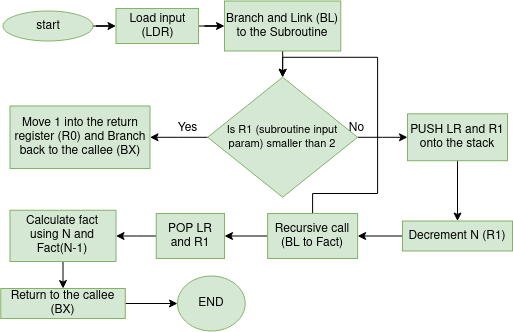
\includegraphics[width=7.5cm]{fact} }}%
    \qquad
    \subfloat[\centering Fibonacci]{{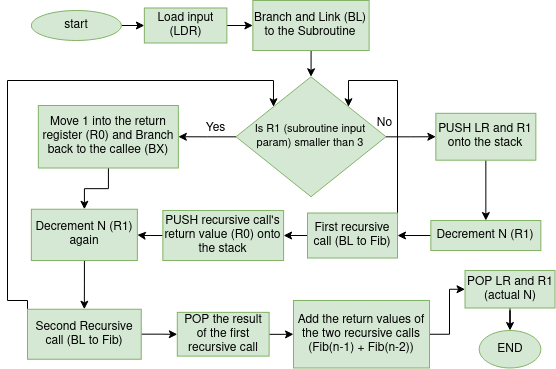
\includegraphics[width=7.5cm]{fib} }}%
    \label{fig:example}%
\end{figure}


\subsection{Factorial}
The factorial of a positive integer $n$ denoted by \textbf{\textit{n!}}, is defined by the product of all positive integers smaller or equal to $n$. For example, $10! = 10 \cdot 9 \cdot 8 \cdot 7 \cdot 6 \cdot 5 \cdot 4 \cdot 3 \cdot 2 \cdot 1 = 3628800 = 0\times375F00$.\\
The implementation summary of the factorial procedure can be found in the flowchart in Figure 1-a.

The program takes an integer $n$ as input. We load this input from memory into the register R1. To follow the ARM Procedure Call Standard (APCS), we choose registers R1 and R0 for passing the parameter $n$, and returning $n!$ to and from the subroutine respectively. Once the input to the subroutine is loaded, we call the factorial subroutine using BL. This instruction branches to the subroutine and stores the address of the next instruction into LR, the link register.\\
The factorial $n!$ is equal to 1 when $n$ is either 1 or 0. For this reason, the factorial subroutine compares the value of $n$ to two. If $n$ is less than two, the subroutine branches to return the number one by storing the value one into R0, the register used for returning values from the factorial procedure. The subroutine then returns to the callee using BX which branches to the address stored previously in the link register LR.\\
If $n$ is greater or equal to two, the recursive part of the subroutine is executed. Before the recursive call to the subroutine, the new input has to be updated by decrementing R1 by one. However, to remember the current value of $n$, which we use later, we push R1 onto the stack. Similarly, to store the address in the link register, which will be overwritten after the subroutine is called recursively using BL, we also push LR onto the stack. Once the recursive step is executed, we pop the value $n$ previously pushed onto the stack and the return address to the callee off the stack. We then store the return value into R0 by multiplying $n$ (R1) by the return value of the recursive call (R0). Finally, the subroutine returns to the callee by branching to the address stored in the link register using BX.
The program then ends by calling an infinite loop. \\

We tested the procedure with values ranging from zero to ten to assure the obtention of correct results. The main challenge we faced in implementing this procedure was the correct usage of the stack, understanding the use of BL and BX instructions, and the call stack.

\subsection{Fibonacci}
Fibonacci numbers create a sequence in which each number is the sum of the two preceding ones. The beginning of the sequence is therefore 0, 1, 1, 2, 3, 5, 8, 13, 21, 34, 55. The procedure to compute the $n^{th}$ Fibonacci number is thus a recursive one of the form Fib(n) = Fib(n-1) + Fib(n-2).\\

The implementation of this procedure is similar in many ways, to the implementation of the factorial procedure described previously. A summary of our implementation can be found in the flowchart in Figure 1-b. We use the ACPS and the Callee-save conventions similarly to the factorial procedure. The main difference between this procedure and the factorial procedure is the presence of not only one but two recursive calls within the subroutine.\\
To begin the program, we load the input $n$ from memory and store it in R1. We use the register R1 to pass the parameter $n$ to the Fibonacci subroutine and the register R0 to store the return value. We then call the Fibonacci subroutine by branching to the subroutine and storing in the load register (LR), the address to the next instruction to run after the subroutine returns using BL.
Similar to the factorial procedure, we compare the input to a number (3 in this case) using CMP to determine whether to return one or to return the result of a recursive call to the subroutine.\\
If $n$ is smaller than three, we return the number one by moving it into R0 and returning to the callee using BX. On the other hand, if $n$ is bigger or equal to 3, we perform the recursive step which consists of two recursive calls. Before performing the first recursive call, we push the current $n$, and LR onto the stack before decrementing $n$ and calling the subroutine using BL. Once the called subroutine returns, we store its return value, stored in R0 onto the stack to be overwritten by the second call's return value.  Once more, we decrement $n$ before performing the second recursive call. After the second call is executed, we pop the result of the first recursive call off the stack, add it to the return value of the second call and store the result of this addition in R0. Lastly, we pop R1 and LR off the stack and the subroutine returns to the callee using BX. The program then ends in an infinite loop.\\

We tested the program's correctness by passing parameters $n$, ranging from zero to twenty. The largest challenge in writing this procedure was to not overwrite registers, especially return values from recursive calls. We overcame this challenge by making efficient use of the stack. The main weakness of this procedure is the recomputation of certain values. For instance in Fib(5) = Fib(4) + Fib(3) and Fib(4) = Fib(3) + Fib(2), Fib(3) is computed twice, significantly reducing time efficiency given larger values of $n$. A better approach would be to use dynamic programming and store computed series to avoid recomputation.
\section{2D Convolution}
In this part, we implement a two-dimensional discrete convolution algorithm defined as a mathematical operation between two functions $f$ and $g$ on an $n$-dimensional lattice. It has many applications, especially in image filters and object detection in machine learning. In this exercise, we perform two-dimensional convolution on a two-dimensional image, given a kernel. Our implementation consists of a deeply nested loop consisting of four loops.\\

Compared to the rest of the programs we wrote in this lab, this program consists of many inputs. We first store all the inputs in the memory. This step consists of storing the flattened two-dimensional image and kernel array and their properties, such as width and height into memory. As we do not perform the convolution in-place, we allocate 400 ($10\times10\times4$) bytes of memory for our output. We then load all program values into registers. However, because this algorithm takes many inputs and consists of many loops, and given that we have a limited number of general-purpose registers in our disposition, we store the memory address of the image, kernel, and output by pushing them onto the stack.\\
For each loop present in our nested loop, we perform the following. First, we initialize the loop counter from its outer loop (or from outside the loop for the main loop) by moving zero into a register. We then check the loop condition using CMP and branch to the outer loop if the condition is not satisfied (we branch to the end of the program for the outmost loop). Otherwise, we increment the loop counter by one and branch back to the loop label.\\
We also initialize a register to hold a sum value calculated in the fourth loop containing the value to write at a certain index of our output array. In our fourth loop, we calculate two temporary values by simple ADD (addition) and SUB (subtraction) instructions. The code given in C contains an if statement in the fourth loop specifying four conditions, all of which have to be true for the statement's body to execute. To implement, we check each condition separately and branch back to the fourth loop after incrementing the loop counter if the condition does not hold; otherwise, we execute the body of the if statement.\\
Once insider the if statement, we realize that all of our 13 general-purpose registers have been used to store loop counters, parameters, and the sum. To overcome this problem, we push registers R0 to R2 into to stack to use them as temporary registers in our calculations. Given that the input arrays are two-dimensional but stored as a one-dimensional array in memory, we perform calculations to find the offset of elements given their row and column index. We find the total offset by summing the row and column offset calculated by multiplying the row index by the row size and the column index by the element size (4 bytes). After retrieving the address to the image and kernel arrays from the stack, we load array contents using the base address and the total offset calculated previously. We then calculate the sum by performing basic arithmetic operations on the array contents. We pop registers R0 to R2 off the stack at the end of the if statement.\\
At the end of the second loop, we store the sum calculated inside the if the statement of the fourth loop into the output array. We retrieve the base address of the output array from the stack and calculate the total offset given row and column indices as described previously. We use this offset and the output array's base address to store the sum value into the correct output location in memory.\\

After the execution of the program, we check that the stack has been restored and emptied. We then analyze the memory contents at the address of the output array to check that correct values were stored at the correct locations.
The main challenge faced was the limited number of registers and the need for more space which was solved by using the stack.
\section{Bubble Sort}
Bubble sort is a simple sorting algorithm that loops through a list and sorts by swapping adjacent elements if they are in the wrong order. In this exercise, we implement Bubble sorting in ascending order in-place.  Its implementation is Assembly requires the usage of branching for implementing loops, memory load, and store to access and modify the input array and comparisons. A summary of our implementation of the bubble sorting algorithm can be found in the flowchart in Figure 2.
\begin{figure}[h]
    \centering
    \caption{Bubble sort flowchart}
    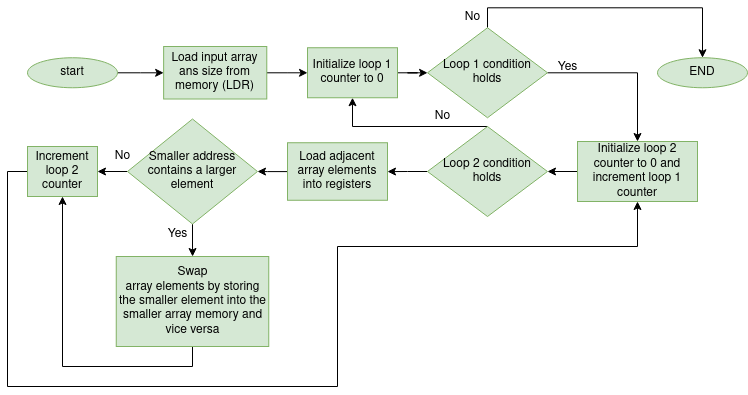
\includegraphics[scale=0.6]{bubblesort}
\end{figure}

We store the input array and its size in the memory. At the start of the program, we load the size of the array and the address of the first element of the array into two registers (R0 and R1 respectively).\\
Next, we implement a nested loop consisting of two loops. To implement the two for loops, we convert them into equivalent while loops, closely resembling Assembly logic. We notice that each loop consists of three steps. The first step is the initialization of the loop counter. The second step consists of checking the condition of the loop counter. The third step simply consists of incrementing the loop counter. For both loops, we initialize the loop counter by moving the value of zero into registers (R2 for loop1 and R3 for loop2) before entering the loop (before the loop label).  Next, we check the loop condition using CMP, and we branch out of the loop if the loop condition doesn't hold. If this condition holds, we increment the loop counter once the loop body is executed and branch back to the loop.\\
We then load adjacent array elements, stored in consecutive memory spaces into two registers, using a scaled index to get the array element at an effective address. We compare the two registers using CMP to update CPSR. We swap array element if an element with a smaller memory address contains a larger value.  We perform this process using STR with a  condition field while employing a scaled index.\\
After the execution of mentioned steps, the array will be sorted by ascending order in-place.\\

We tested the implemented sorting algorithm by passing arrays, both presorted and unsorted, with different sizes containing positive and negative values.
Implementing the bubble sort algorithm is not particularly challenging. However, grasping memory load and store instructions are challenging at first. Being very simple to implement, bubble sort is extremely time inefficient. While testing the program with presorted arrays, the algorithm performed as many steps as when the input array was sorted in reverse order. We became interested in reducing the number of taken steps by the algorithm when the input array is already perfectly or mostly sorted. \\

Nevertheless, some optimizations can significantly improve the bubble sort's performance that we didn't implement. After each iteration, if no swapping takes place, there is no need to perform further loops. Thus, introducing an extra variable that keeps track of whether elements were swapped in an iteration and stopping the sorting when no swapping happens can significantly improve the efficiency of the algorithm, especially when the input array is already correctly sorted.

\end{document}
